% Original book diagram: fig:autonomous_infrastructure_loop
% Book source: sections/Part_VI/infrastructure_applications.tex
% Original diagram authorship retained. Visual design: Ziad Mosalam.
\documentclass[11pt,border=8pt]{standalone}
\usepackage{amsmath,amssymb,graphicx,tikz}
\usetikzlibrary{arrows.meta,automata,positioning,calc,shapes.geometric,fit,backgrounds,patterns}
\newcommand{\vect}[1]{\mathbf{#1}}
\newcommand{\mat}[1]{\mathbf{#1}}
\newcommand{\Normal}{\mathcal{N}}
\newcommand{\prob}{p}
\newcommand{\E}{\mathbb{E}}
\newcommand{\Var}{\mathrm{Var}}
\newcommand{\Cov}{\mathrm{Cov}}
\newcommand{\CovP}{\mathbf{P}}
\newcommand{\Prob}{\mathbb{P}}
\setlength{\textwidth}{6.5in}
% Shared visual vocabulary for the book's original diagrams.
% Figures opt in explicitly, so unrelated text and existing additions are unchanged.
\definecolor{BookBlue}{HTML}{003262}
\definecolor{BookGold}{HTML}{B17A00}
\definecolor{BookTeal}{HTML}{247C86}
\definecolor{BookInk}{HTML}{30363B}
\definecolor{BookLight}{HTML}{E9EFF5}
\tikzset{
  book figure/.style={font=\small\rmfamily, color=BookBlue, text=BookInk,
    line width=0.8pt, >=Latex},
  book axis/.style={->, draw=BookInk, line width=0.6pt},
  book link/.style={->, draw=BookBlue, line width=0.8pt},
  book observation/.style={draw=BookGold, fill=BookGold!8},
  book state/.style={draw=BookBlue, fill=BookLight},
  book note/.style={font=\footnotesize\rmfamily, text=BookInk}
}

\begin{document}
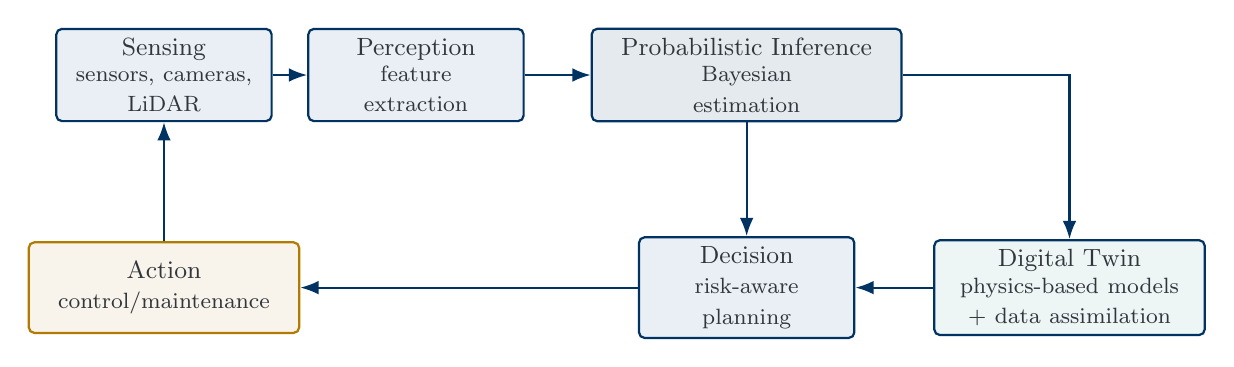
\begin{tikzpicture}[book figure,
    >=Latex,
    block/.style={
        rectangle,
        draw,
        rounded corners=2pt,
        text width=2.5cm,
        minimum height=1.15cm,
        align=center,
        line width=0.8pt,
        fill=BookLight,
        font=\small
    },
    inference/.style={block, fill=BookBlue!10, text width=3.7cm},
    action/.style={block, draw=BookGold, fill=BookGold!8, text width=3.2cm},
    twin/.style={
        rectangle,
        draw,
        rounded corners=2pt,
        text width=3.2cm,
        minimum height=1.15cm,
        align=center,
        line width=0.8pt,
        fill=BookTeal!8,
        font=\small
    },
    arrow/.style={->, draw=BookBlue, line width=0.8pt}
]

% Top row
\node[block] (sense) at (0,2)
    {Sensing\\{\footnotesize sensors, cameras,\\LiDAR}};
\node[block] (perception) at (3.2,2)
    {Perception\\{\footnotesize feature\\extraction}};
\node[inference] (inference) at (7.4,2)
    {Probabilistic Inference\\{\footnotesize Bayesian\\estimation}};

% Bottom row
\node[action] (action) at (0,-.7)
    {Action\\{\footnotesize control/maintenance}};
\node[block] (decision) at (7.4,-.7)
    {Decision\\{\footnotesize risk-aware planning}};
\node[twin] (twin) at (11.5,-.7)
    {Digital Twin\\{\footnotesize physics-based models\\+ data assimilation}};

% Main pipeline
\draw[arrow] (sense.east) -- (perception.west);
\draw[arrow] (perception.east) -- (inference.west);
\draw[arrow] (inference.south) -- (decision.north);
\draw[arrow] (decision.west) -- (action.east);

% Digital-twin connections
\draw[arrow] (inference.east) -| (twin.north);
\draw[arrow] (twin.west) -- (decision.east);

% Feedback from action to sensing
\draw[arrow] (action.north) -- (sense.south);

\end{tikzpicture}
\end{document}
